\documentclass[10pt,a4paper]{article}
\newcommand{\judul}{Modul Bunyi}
\newcommand{\penulis}{bintangpelajar.com}
\usepackage[latin1]{inputenc}
\usepackage{amsmath}
\usepackage{microtype}
\usepackage[none]{hyphenat}
\usepackage{verbatim}
\usepackage{amsfonts}
\usepackage{amssymb}
\usepackage{enumitem}
\renewcommand{\familydefault}{\sfdefault}
\usepackage{mathpazo}
\renewcommand{\rmdefault}{put}
\usepackage{enumitem}
\usepackage[dvipsnames,svgnames]{xcolor}
\usepackage{tkz-euclide}
\usetkzobj{all}
\usepackage{graphicx}
\usepackage{fancyhdr}
\usepackage{tikz} 	
\usepackage{adjustbox}
\usepackage{multicol}
\usepackage{lipsum}
\usepackage[headsep=0.2cm,footskip=0.5cm,left=0.3cm,right=0.7cm,top=1.7cm,bottom=1.0cm]{geometry}
\usepackage{cancel} \usepackage{xcolor}
\usepackage{tcolorbox}
\usetikzlibrary{decorations.pathmorphing,patterns}
\usetikzlibrary{decorations.pathreplacing,calc}
 \newcommand\coret[2][red]{\renewcommand\CancelColor{\color{#1}}\cancel{#2}}
\SetLabelAlign{Center}{\hfil\makebox[1.0em]{#1}\hfil}

\newtcolorbox{mybox}[1][] { colframe = blue!10, colback = blue!3,boxsep=0pt,left=0.2em, coltitle = blue!20!black, title = \textbf{jawab}, #1, } 

%---------- kunci (jika 1 ) muncul
\def\tampilkunci{1}
\newcommand{\hide}[1]{\ifnum\tampilkunci=1
%
\begin{mybox}
 #1
\end{mybox}
%
%\vspace{\baselineskip}
\fi}

\newcommand*\cicled[1]{\tikz[baseline=(char.base)]{\node[white, shape=circle, fill=red!80,draw,inner sep=0.5pt](char){#1};}}

\newcommand*\kunci[1]{\ifnum\tampilkunci=1
%
\tikz[baseline=(char.base)]{\node[red, shape=circle,draw,inner sep=0.5pt,xshift=2pt](char){#1};}\stepcounter{enumii}
\fi\ifnum\tampilkunci=0
%
\hspace{3pt}#1\stepcounter{enumii}
%
\fi}

%------------- MULAI FUNGSIKU ------------
\newcommand{\cartesius}[3]{
\draw[help lines] (-1,-1) grid (#1);
\foreach \x in {1,2,...,#2}{
\node at (\x,0)[scale=0.5]{\x};}
\foreach \y in {1,2,...,#3}{
\node at (0,\y) [scale=0.5]{\y};}}

\newcommand{\pers}[1]{\begin{align*} #1 \end{align*}}
% \sci{ }  misal  x 10^2  tinggal tulis 
% \sci{2} 
\newcommand{\sci}[1]{$\times 10^{#1}$}

\newcommand{\scip}[1]{\times 10^{#1}}

%----membuat tanda silang di samping text
\newcommand*\silang[1]{\tikz[baseline=(char.base)]{
\draw[red,thick](-0.2,-0.20)--(0.2,0.2);
\draw[red,thick](-0.2,0.20)--(0.2,-0.2);
\node[black](char){#1};
}}
%----- membuat tanda centang di mana saja
\newcommand*\centang[1]{\tikz[baseline=(char.base)]{
\draw[red, very thick](-0.2,0.1)--(-0.1,0)--(0.2,0.3);
\node(char){#1};
}}
%------------mewarnai text merah
\newcommand*\merah[1]{
\textcolor{red}{#1}}
\newcommand*\pilgan[1]{
\begin{enumerate}[label=\Alph*., itemsep=0pt,topsep=0pt,leftmargin=*,align=Center] #1 
\end{enumerate}}

%---- membuat pernyataan pada soal SBMPTN
\newcommand*\pernyataan[1]{
\begin{enumerate}[label=(\arabic*), itemsep=0pt,topsep=0pt,leftmargin=*] #1 
\end{enumerate}}

%------ lebar baris pada tabular
\newcommand{\baris}[1]{\renewcommand\arraystretch{#1} }
%\newcommand{\tabel}[2j]{\begin{tabular}{#1}
%\end{tabular}
%------------ END OF FUNGSIKU ----------- 

\newcommand{\pilgani}[1]{
\vspace{-0.3cm}\begin{multicols}{2}
 \begin{enumerate}[label=\Alph*., itemsep=0pt,topsep=0pt,leftmargin=*,align=Center]#1
\end{enumerate}
\phantom{ini cuma sapi, wedus, dan ayam}
\end{multicols}}

%--------------- begin{document}-----------
\pagestyle{fancy}
\fancyhf{} 
\rhead{\penulis}
\lhead{\judul}
\rfoot{Hal \thepage}
\begin{document}


\begin{multicols*} {2} 
\begin{enumerate}[itemsep=0mm]

%------------ nomor 1----------
%  UMPTN 1998
\item Perhatikan diagram berikut!


Di dalam 2 bejana di atas masing-masing berisis zat cair yang perbandingan masa jeninya $\rho_A$ : $\rho_B$ = 5:4 . Titik pada bejana A yag mempunyai tekanan sama dengan titik P pada bejana B adalah titik . . . .
\pilgani{\small{
\item (5), $h_5$ = 8cm
\item (4), $h_4$ = 10cm
\item (3), $h_3$ = 12cm
\item [\kunci{D.}] (2), $h_2$ = 16cm
\item (1), $h_1$ = 20cm
}}

%--------------- nomor 2 ------------
% UNSMK 2004
\item Air di dalam tabung mempunyai masa jenis 1 gram cm$^3$. Tekanan hidrostatis di titik B (lihat pada gambar), bila titik B berada pada kedalaman 20 cm dari permukaan dan $g$ = 10 m/s$^2$ adalah . . .

\begin{minipage}{0.19\textwidth}
\pilgan{
\item [\kunci{A.}]2 \sci{3} N/m$^2$
\item 3 \sci{3} N/m$^2$
\item 4 \sci{3} N/m$^2$
\item 5 \sci{3} N/m$^2$
\item 6 \sci{3} N/m$^2$
}
\end{minipage}\begin{minipage}{0.13\textwidth}
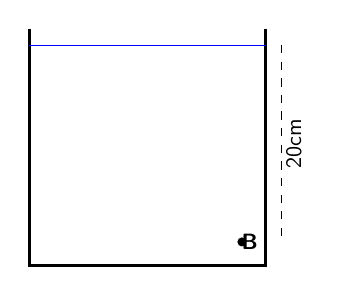
\begin{tikzpicture}
\draw[very thick](0,3)--(0,0)--(3,0)--(3,3);
\draw[dashed] (3.2,2.8) -- node [midway,scale=0.8, rotate=90, yshift=-0.2cm]{20cm}(3.2,0.3);
\draw [fill=black](2.7,0.3)circle(0.05cm);
 \node at (2.8,0.3)[scale=0.8]{\textbf{B}};
\draw[thin,blue](0,2.8)--(3,2.8);
\end{tikzpicture}\end{minipage}

\hide{
\pers{
p_h &= \rho.g.h\\
p_h &= 1000.10.0,2\\
p_h &= 2 \scip{3} \text{ N/m}^2}
}

%------------------- nomor 3 ------
% UAN SMK 2002
\item Bendungan menampung air setinggi 80 meter. (massa jenis air 1000 kg/m$^3$, $g$ = 10 m/s$^2$). Besar tekanan hidrostatis pada suatu titik yang berada di 60 m di bawah permukaan air adalah . . . 
\pilgani{
\item 6 \sci{4} N/m$^2$
\item 8 \sci{4} N/m$^2$
\item 2 \sci{5} N/m$^2$
\item [\kunci{D.}]6 \sci{5} N/m$^2$
\item 8 \sci{5} N/m$^2$
}\hide{
untuk menghitung tekanan hidrostatis menggunakan persamaan $p_h=\rho.g.h$ di mana $h$ adalah kedalaman dari permukaan. maka jawaban soal ini adalah
\pers{
p_h&=\rho.g.h\\
p_h&=1000.10.60\\
p_h&=6\scip{5}\text{ N/m}^2}}


%------------ nomor 4 -----------
% UN SMK 2004
\item Seorang penyelam memeriksa kerangka kapal laut pada kedalaman 15 m di bawah permukaan air. Bila $g$ = 9.8 m/s$^2$ dan massa jenis air laut 1100 kg/m$^3$, maka tekanan hidrostatis yang dialami penyelam adalah . . .
\pilgani{
\item 161.700 N/m$^2$
\item 16.500 N/m$^2$
\item 10.780 N/m$^2$
\item 719 N/m$^2$
\item 147 N/m$^2$
}



%----------------- nomor 5 ----------
% EBTANAS 1993 
\item Gambar bejana berhubungan yang berisi air. Tekanan hidrostatis yang paling besar berada di titik . . . .

\pilgani{
\item P
\item Q
\item R
\item S
\item [\kunci{E.}]T
}

%----------------- nomor 6 ----------
% EBTANAS 1995
\item Dua buah bejana A dan B diisi dengan zat cair yang berbeda massa jennisnya terlihat seperti gambar. Perbandingan massa jenis zat cair di A dibandingkan dengan massa jenis zat cair di B adalah 3:4.



Titik di tabung B yang mempunyai tekanan yang sama dengan tekanan pada dasar tabung A adalah . .. .
\pilgan{
\item [\kunci{A.}]P
\item Q
\item R
\item S
\item T
}
\hide{
Pada soal ditanyakan adalah lokasi (kedalaman) di B yang tekanannya sama saat kedalama A adalah 80.
\pers{
p_A &= p_B \\
\rho_A.g.h_A &= \rho_B.g.h_B\\
3.10.80 &= 4.10.h_B\\
60 &= h_B}
Jadi kedalaman B di 60 dari permukaan, yakni di titik P.}


%----------------- nomor 7 ------------
%   EBTANAS 1990
\item Raksa pada bejana berhubungan mempunyai selisih 2 cm (massa jenis 13,6 g/cm$^3$). Kaki sebelah kiri berisi zat cair yang tingginya 25 cm, berarti massa jenis zat cair itu adalah . . .

\begin{minipage}{0.18\textwidth}
\pilgan{
\item 800 kg/m$^3$
\item 1030 kg/m$^3$
\item [\kunci{C.}]1088 kg/m$^3$
\item 1300 kg/m$^3$
\item 1360 kg/m$^3$
} \end{minipage}\begin{minipage}{0.20\textwidth}
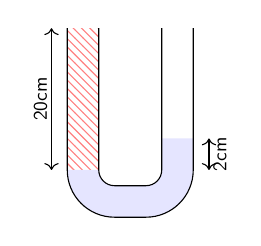
\begin{tikzpicture}[scale=0.2]
%\draw[help lines](0,0)grid(12,16);
\fill [pattern=north west lines, pattern color=red!50] (3,3) rectangle (5,12);
\fill[blue!10] (11,5)--(11,3) arc [start angle=0, end angle=-90, radius=3]--++(-2,0)arc [start angle=270, end angle=180,radius=3]--++(2,0)arc [start angle=180,end angle = 270, radius=1]--++(2,0) arc [start angle=270, end angle=360,radius=1]--++(0,2)++(2,0);
\draw(11,12)--(11,3) arc [start angle=0, end angle=-90, radius=3]--++(-2,0)arc [start angle=270, end angle=180,radius=3]--++(0,9)++(2,0)--++(0,-9)arc [start angle=180,end angle = 270, radius=1]--++(2,0) arc [start angle=270, end angle=360,radius=1]--++(0,9)++(2,0)--++(0,-9);
\draw [<->] (12,3) -- (12,5) node [midway,rotate=90, scale=0.7, yshift=-0.2cm]{2cm};
\draw [<->] (2,3)--(2,12) node [midway,rotate=90,scale=0.7, yshift=0.2cm]{20cm};
\end{tikzpicture}
\end{minipage}
\hide{
Untuk mengerjakan soal ini, raksa memiliki tinggi 2cm dan tinggi zat cair 25 cm.Besarnya tekanan pada titik perbatasan dengan titik di kaki kanan tabung adalah sama. 
\pers{
p_r &= p_c\\
\rho_r.g.h_r &= \rho_c.g.h_c\\
13600.10.2 &= \rho_c.10.25\\
\rho_c &= 1088 \text{ kg/m}^3
}
}

%----------- nomor 8 
% EBTANAS 1996 (prog.A2)
\item Pada gambar di bawah, pipa berbentuk U diisi air dan oli ($\rho_{\text{air}}$ = 1 g/cm$^3$, $\rho_{\text{oli}}$ = 0,8 g/cm$^3$). Selisih tinggi permukaan air dan oli adalah . . . 

\begin{minipage}{0.18\textwidth}
\pilgan{
\item 1,6 cm
\item 3,2 cm
\item 4 cm
\item 5 cm
\item 16 cm
} \end{minipage}\begin{minipage}{0.20\textwidth}
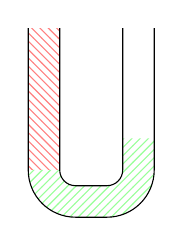
\begin{tikzpicture}[scale=0.2]
%\draw[help lines](0,0)grid(12,16);
\fill [pattern=north west lines, pattern color=red!50] (3,3) rectangle (5,12);
\fill[pattern=north east lines,pattern color=green!40] (11,5)--(11,3) arc [start angle=0, end angle=-90, radius=3]--++(-2,0)arc [start angle=270, end angle=180,radius=3]--++(2,0)arc [start angle=180,end angle = 270, radius=1]--++(2,0) arc [start angle=270, end angle=360,radius=1]--++(0,2)++(2,0);
\draw(11,12)--(11,3) arc [start angle=0, end angle=-90, radius=3]--++(-2,0)arc [start angle=270, end angle=180,radius=3]--++(0,9)++(2,0)--++(0,-9)arc [start angle=180,end angle = 270, radius=1]--++(2,0) arc [start angle=270, end angle=360,radius=1]--++(0,9)++(2,0)--++(0,-9);

\end{tikzpicture}
\end{minipage}



%--------------- nomor 9
% EBTANAS 1995 
\item Perhatikan gambar berikut ini !


Bila diketahui $m_B$ = 6 ton dan $g$ = 10 m/s$^2$ maka massa beban A ($m_A$) adalah . . .
\pilgani{
\item 2 kg
\item 3 kg
\item 4 kg
\item 5 kg
\item 6 kg
}


% ------------- nomor 10
% SPMB 2003
\item Pengisap P mempunyai luas penampang 0,75 cm$^2$ yang bergerak bebas tanpa gesekan sehingga dapat menekan pegas sejauh $\Delta x$. Jika konstanta pegas 75 N/m dan massa jenis zat cair 500 kg/m$^3$, maka $\Delta x$ adalah. . . .

\begin{minipage}{0.18\textwidth}
\pilgan{
\item 0,4 cm
\item 0,5 cm
\item 0,6 cm
\item 0,7 cm
\item 1 cm
} \end{minipage}\begin{minipage}{0.20\textwidth}
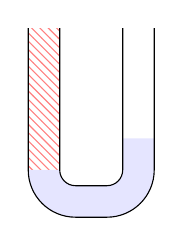
\begin{tikzpicture}[scale=0.2]
%\draw[help lines](0,0)grid(12,16);
\fill [pattern=north west lines, pattern color=red!50] (3,3) rectangle (5,12);
\fill[blue!10] (11,5)--(11,3) arc [start angle=0, end angle=-90, radius=3]--++(-2,0)arc [start angle=270, end angle=180,radius=3]--++(2,0)arc [start angle=180,end angle = 270, radius=1]--++(2,0) arc [start angle=270, end angle=360,radius=1]--++(0,2)++(2,0);
\draw(11,12)--(11,3) arc [start angle=0, end angle=-90, radius=3]--++(-2,0)arc [start angle=270, end angle=180,radius=3]--++(0,9)++(2,0)--++(0,-9)arc [start angle=180,end angle = 270, radius=1]--++(2,0) arc [start angle=270, end angle=360,radius=1]--++(0,9)++(2,0)--++(0,-9);

\end{tikzpicture}
\end{minipage}


\end{enumerate}
\end{multicols*}

 \end{document}
